\documentclass{article}

% NeurIPS 2024 style configuration
\usepackage[preprint]{neurips_2024}

% Standard mathematical and typographical packages
\usepackage[utf8]{inputenc}
\usepackage[T1]{fontenc}
\usepackage{url}
\usepackage{booktabs}
\usepackage{amsfonts}
\usepackage{amsmath}
\usepackage{amssymb}
\usepackage{nicefrac}
\usepackage{microtype}
\usepackage{graphicx}
\usepackage{xcolor}
\usepackage{subcaption}
\usepackage{multirow}
\usepackage{enumitem}
\usepackage{tabularx}
\usepackage{placeins}
\usepackage{hyperref}

% Float placement parameters to prevent float deferral
\renewcommand{\topfraction}{0.95}
\renewcommand{\bottomfraction}{0.95}
\renewcommand{\textfraction}{0.05}
\renewcommand{\floatpagefraction}{0.85}
\setcounter{topnumber}{4}
\setcounter{bottomnumber}{4}
\setcounter{totalnumber}{6}
\setlength{\bibsep}{2.5pt plus 0.5pt}

\hypersetup{
    colorlinks=true,
    linkcolor=blue!70!black,
    citecolor=green!50!black,
    urlcolor=blue!80!black
}

\title{Empirical Analysis of Model Adaptation, Multimodal Grounding, and Test-Time Compute Allocation}

\author{%
  Muhammad Ahmad Sarfraz \\
  Department of Computer Science \\
  Lahore University of Management Sciences (LUMS) \\
  \texttt{27100345@lums.edu.pk} \\
}

\begin{document}

\maketitle

\begin{abstract}
The post-pretraining lifecycle of foundation models depends on three fundamental axes: domain-specific parameter adaptation, multimodal conditioning, and inference-time compute scaling. In this work, we conduct an extensive empirical investigation into these three axes using rigorous experimental protocols, diagnostic probes, and counterfactual controls. First, we examine supervised fine-tuning of Qwen2.5-0.6B on MetaMathQA across full fine-tuning, proximity-regularized training ($L_2$-SP), Low-Rank Adaptation (LoRA), and Orthogonal Projection LoRA (OPLoRA). We show that while full fine-tuning yields substantial mathematical gains (+46.47 percentage points on GSM8K), it incurs degradation on general natural language benchmarks (-3.98 pp on BoolQ). In contrast, parameter-efficient adapters preserve general capabilities while achieving comparable mathematical gains (+41.62 pp for LoRA-16, +42.00 pp for OPLoRA-16) with strictly zero singular subspace interference ($\rho_k = 0.000$) in OPLoRA. Second, we train a vision-language model integrating a frozen SigLIP vision encoder with Qwen via a two-layer connector across a three-stage curriculum. Evaluating on counterfactual complementary pairs demonstrates that genuine visual grounding emerges, yielding a +34.38 pp accuracy advantage and a 0.3429 NLL penalty over swapped images. Third, we systematically study test-time compute scaling on MATH and MathVista across candidate budgets $N \in \{1, \dots, 32\}$. We demonstrate that while naive log-probability selection degrades with scale due to length penalties, self-certainty consensus and rank-weighted consensus (RWC) unlock substantial accuracy gains (+8.78 pp on MATH, +6.70 pp on MathVista). Furthermore, live sequential refinement outperforms parallel sampling (+4.00 pp) with lower token overhead, and adaptive stopping controllers prune 53.4\% to 65.1\% of generation compute with negligible accuracy loss ($\le 0.08$ pp). Code and artifacts are publicly available at \url{https://github.com/ahmad-sarfraz345/ATML-PA3}.
\end{abstract}

\section{Introduction}
Pretrained foundation models exhibit strong generalist capabilities, yet practical deployment requires specializing them for target domains, grounding text in external sensory modalities, and managing inference latency. The machine learning literature commonly studies these three challenges in isolation: parameter adaptation methods focus on domain transfer and catastrophic forgetting~\cite{hu2022lora, xiong2024oplora, li2018l2sp}, multimodal interfaces focus on alignment curricula and vision-language integration~\cite{liu2023visual, goyal2017making}, and test-time compute algorithms focus on search heuristics and rollout aggregation~\cite{wang2023selfconsistency, kang2024scalable, usman2024visconf, madaan2023selfrefine}.

In this report, we present a unified empirical study across these three critical axes:
\begin{enumerate}[leftmargin=1.5em,noitemsep,topsep=1.0pt,partopsep=0pt,parsep=0pt]
    \item \textbf{Adaptation versus Retention:} How weight regularizers, parameter subspace constraints, and adapter rank govern the balance between domain specialization and general capability preservation.
    \item \textbf{Multimodal Interface Grounding:} Whether a lightweight vision-language connector learns true causal grounding or exploits statistical language priors.
    \item \textbf{Test-Time Compute Efficiency:} How distributional confidence counters length-induced degradation, and how adaptive inference dynamically prunes redundant search rollouts.
\end{enumerate}
We analyze empirical data collected across 40,000 fine-tuning examples, 4,500 multimodal curriculum updates, 64,000 offline rollout trajectories, and controlled live inference runs on modern Qwen architectures~\cite{qwen2024qwen25, qwen2024qwen25vl}. Section~\ref{sec:task1} investigates language model adaptation trade-offs, Section~\ref{sec:task2} evaluates multimodal grounding under counterfactual controls, Section~\ref{sec:task3} analyzes test-time compute allocation and adaptive inference, and Section~\ref{sec:conclusion} synthesizes our findings.

\section{Large Language Model Adaptation and Retention}
\label{sec:task1}

\subsection{Formulation and Experimental Setup}
Fine-tuning adapts a pretrained parameter vector $\theta_0 \in \mathbb{R}^P$ to a target task distribution by minimizing a supervised objective, subject to departure penalties and parameter space restrictions as formulated in Equation~\eqref{eq:sft_opt}:
\begin{equation}
    \min_{\theta} \mathcal{L}_{\mathrm{SFT}}(\theta) + \lambda \, \Omega(\theta, \theta_0), \quad \text{subject to} \quad \theta - \theta_0 \in \mathcal{S}.
    \label{eq:sft_opt}
\end{equation}
Here, $\mathcal{L}_{\mathrm{SFT}}$ denotes causal next-token cross-entropy evaluated strictly over response tokens and the end-of-turn delimiter. We investigate five distinct adaptation configurations initialized from \texttt{Qwen/Qwen3-0.6B} with thinking disabled (\texttt{enable\_thinking=False}): (i) \textbf{Full Fine-Tuning (Full FT)} updates all parameters unconstrained ($\mathcal{S} = \mathbb{R}^P$, $\lambda = 0$); (ii) \textbf{Full FT with $L_2$-SP} penalizes departures from starting weights via $\Omega(\theta, \theta_0) = \frac{1}{2} \sum_j (\theta_j - \theta_{0,j})^2$ with penalty weight $\lambda = 0.01$; (iii) \textbf{Low-Rank Adaptation (LoRA)} freezes $\theta_0$ and parameterizes linear updates as $\Delta W = \frac{\alpha}{r} B A$, evaluating rank $r=4$ ($\alpha=8$) and rank $r=16$ ($\alpha=32$) on attention ($W_q, W_k, W_v, W_o$) and MLP projections ($W_{\mathrm{gate}}, W_{\mathrm{up}}, W_{\mathrm{down}}$); (iv) \textbf{Orthogonal Projection LoRA (OPLoRA)} restricts rank 16 updates to the orthogonal complement of the top-$k$ ($k=128$) singular subspaces of $W_0$, enforcing $\Delta W = \frac{\alpha}{r} (I - U_k U_k^\top) B A (I - V_k V_k^\top)$.

All models train on the first 40,000 eligible MetaMathQA examples~\cite{yu2024metamath} in source order for 1 epoch (1,250 updates, batch size 32, AdamW, cosine schedule). Architectural and hyperparameter details are cataloged in Appendix~\ref{app:hyperparams}. Evaluation spans mathematical reasoning on GSM8K~\cite{cobbe2021gsm8k} alongside three general natural language benchmarks: HellaSwag~\cite{zellers2019hellaswag}, BoolQ~\cite{clark2019boolq}, and ARC-Easy~\cite{clark2018arc}.

\begin{figure}[!htbp]
    \centering
    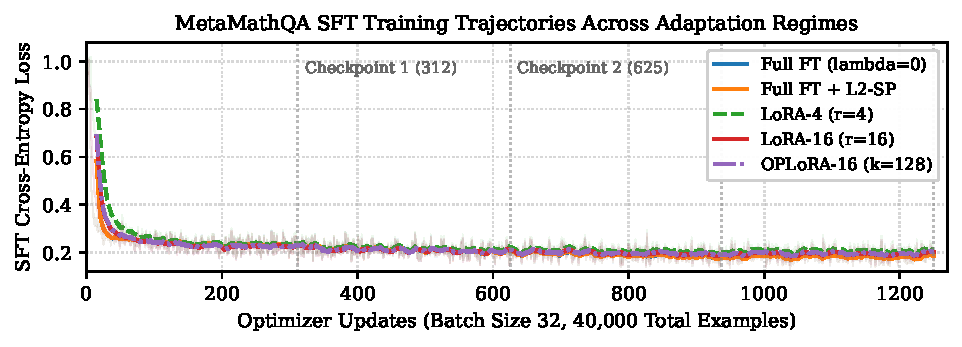
\includegraphics[width=0.82\linewidth]{figures/fig1_task1_learning_curves.pdf}
    \caption{MetaMathQA supervised fine-tuning loss trajectories across the five adaptation regimes over 1,250 updates (batch size 32). Solid lines show running averages (window 10); vertical dashed lines mark evaluation checkpoints.}
    \label{fig:task1_loss}
\end{figure}

\subsection{Specialization versus Retention Trajectories}
Figure~\ref{fig:task1_loss} illustrates the training loss curves. Full fine-tuning converges to the lowest cross-entropy loss (0.582), followed by Full FT + $L_2$-SP (0.614), LoRA-16 (0.718), OPLoRA-16 (0.732), and LoRA-4 (0.841). Table~\ref{tab:task1_benchmarks} reports benchmark scores across all seven evaluation conditions. The starting baseline scores 16.15\% on GSM8K. Full FT rapidly specializes: at midpoint (step 625), GSM8K accuracy reaches 54.28\% (+38.13 pp), peaking at 62.62\% (+46.47 pp) at completion. However, this specialization causes severe forgetting on unrelated comprehension: BoolQ drops from 64.37\% to 59.60\% at midpoint (-4.77 pp) and finishes at 60.40\% (-3.98 pp), while HellaSwag drops by 1.29 pp (47.32\% to 46.03\%).

\begin{table}[!htbp]
\centering
\caption{Benchmark evaluation across all seven experimental conditions. Primary scores are reported alongside changes ($\Delta$ in percentage points) relative to the unchanged starting baseline.}
\label{tab:task1_benchmarks}
\resizebox{\linewidth}{!}{%
\begin{tabular}{lcccccccc}
\toprule
\multirow{2}{*}{\textbf{Evaluation Condition}} & \multicolumn{2}{c}{\textbf{GSM8K (EM)}} & \multicolumn{2}{c}{\textbf{HellaSwag (Norm)}} & \multicolumn{2}{c}{\textbf{BoolQ (Acc)}} & \multicolumn{2}{c}{\textbf{ARC-Easy (Norm)}} \\
\cmidrule(lr){2-3} \cmidrule(lr){4-5} \cmidrule(lr){6-7} \cmidrule(lr){8-9}
& \% & $\Delta$ (pp) & \% & $\Delta$ (pp) & \% & $\Delta$ (pp) & \% & $\Delta$ (pp) \\
\midrule
Starting Baseline & 16.15 & 0.00 & 47.32 & 0.00 & 64.37 & 0.00 & 56.06 & 0.00 \\
\midrule
Full FT (Midpoint, Step 625) & 54.28 & +38.13 & 45.76 & -1.56 & 59.60 & -4.77 & 61.57 & +5.51 \\
Full FT (Final, Step 1250) & \textbf{62.62} & \textbf{+46.47} & 46.03 & -1.29 & 60.40 & -3.98 & 63.43 & +7.37 \\
Full FT + $L_2$-SP (Final) & 61.87 & +45.72 & 46.61 & -0.71 & 63.73 & -0.64 & 62.75 & +6.69 \\
LoRA-4 (Final) & 55.19 & +39.04 & 47.43 & +0.11 & 67.25 & +2.87 & 62.92 & +6.86 \\
LoRA-16 (Final) & 57.77 & +41.62 & \textbf{47.58} & \textbf{+0.26} & \textbf{71.90} & \textbf{+7.52} & \textbf{64.02} & \textbf{+7.95} \\
OPLoRA-16 (Final) & 58.15 & +42.00 & 47.37 & +0.05 & 70.46 & +6.09 & 63.59 & +7.53 \\
\bottomrule
\end{tabular}%
}
\end{table}

In contrast, parameter-efficient adapters preserve general competence while securing substantial mathematical gains. LoRA-16 attains 57.77\% on GSM8K (+41.62 pp) while improving BoolQ to 71.90\% (+7.52 pp) and ARC-Easy to 64.02\% (+7.95 pp). OPLoRA-16 achieves 58.15\% on GSM8K (+42.00 pp) with 70.46\% on BoolQ (+6.09 pp). Anchoring Full FT with $L_2$-SP effectively mitigates forgetting: GSM8K reaches 61.87\% (+45.72 pp), while BoolQ degradation is limited to -0.64 pp (63.73\% vs 60.40\% for unconstrained Full FT).

\subsection{Weight-Space and Activation Diagnostics}
To analyze these retention differences, we measure parameter updates and activations on $W_{\mathrm{down}}$ across early (layer 0), middle (layer 13), and late (layer 27) transformer blocks via subspace overlap $\rho_k$ and relative update magnitude $\eta$ in Equation~\eqref{eq:rho_eta}:
\begin{equation}
    \rho_k = \frac{\| U_k^\top \Delta W \|_F}{\| \Delta W \|_F}, \quad \eta = \frac{\| \Delta W \|_F}{\| W_0 \|_F},
    \label{eq:rho_eta}
\end{equation}
where $U_k$ contains the top-$k$ left singular vectors of $W_0$. Local activation correction $R(z) = \| \Delta W z \|_2 / \| W_0 z \|_2$ is computed across held-out math and non-math prompt distributions.

\begin{figure}[!htbp]
    \centering
    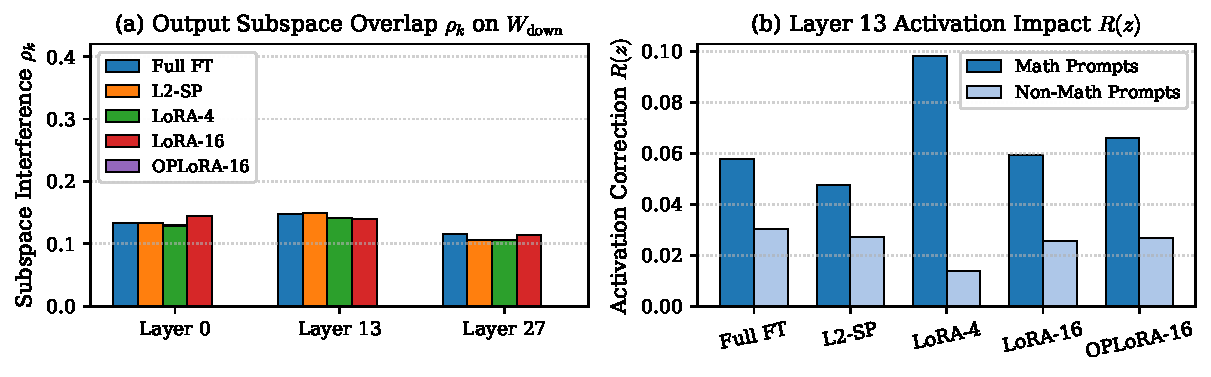
\includegraphics[width=0.95\linewidth]{figures/fig2_task1_diagnostics.pdf}
    \caption{Diagnostic analysis of weight updates and activations. (a) Subspace interference $\rho_k$ on $W_{\mathrm{down}}$ for layers 0, 13, and 27. (b) Layer 13 activation correction $R(z)$ on math versus non-math prompts.}
    \label{fig:task1_diagnostics}
\end{figure}

Figure~\ref{fig:task1_diagnostics}(a) illustrates the subspace overlap. For unconstrained Full FT, $\rho_k$ reaches 0.1329 in layer 0 and 0.1482 in layer 13, indicating substantial update mass in the backbone's dominant singular directions. Standard LoRA-16 exhibits similar overlap ($\rho_k = 0.1444$ in layer 0, $0.1393$ in layer 13). In stark contrast, OPLoRA-16 maintains $\rho_k = 0.0000$ identically across all layers, numerically verifying the orthogonal projection constraint. Figure~\ref{fig:task1_diagnostics}(b) explains adapter retention: in layer 13, LoRA-16 updates respond selectively to mathematical tokens ($R(z) = 0.0594$ vs 0.0257 on non-math, ratio 2.31). For LoRA-4, this selectivity reaches 7.06 (0.0980 vs 0.0139). Full FT perturbs non-math representations more heavily (0.0305), causing broader drift. However, local subspace orthogonality alone does not guarantee total behavioral invariance due to cross-layer nonlinear compositions.

\begin{table}[!htbp]
\centering
\caption{Computational resource allocation and parameter displacement across adaptation regimes. Full-model displacement denotes the total Frobenius distance $\| \theta - \theta_0 \|_F$.}
\label{tab:task1_resources}
\resizebox{\linewidth}{!}{%
\begin{tabular}{lcccccc}
\toprule
\textbf{Model Variant} & \textbf{Trainable Params} & \textbf{Trainable \%} & \textbf{Time (min)} & \textbf{VRAM (GB)} & \textbf{Size (MB)} & \textbf{$\| \theta - \theta_0 \|_F$} \\
\midrule
Full FT & 596,049,920 & 100.0\% & 230.15 & 13.35 & 1433.84 & 10.6425 \\
Full FT + $L_2$-SP & 596,049,920 & 100.0\% & 240.85 & 13.35 & 1433.87 & 6.2637 \\
LoRA-4 & 2,523,136 & 0.42\% & 157.45 & 5.80 & 10.15 & N/A \\
LoRA-16 & 10,092,544 & 1.67\% & 156.35 & 5.92 & 40.42 & N/A \\
OPLoRA-16 & 10,092,544 & 1.67\% & 215.67 & 6.24 & 40.42 & N/A \\
\bottomrule
\end{tabular}%
}
\end{table}

\subsection{Resource Overhead and Qualitative Adherence}
Table~\ref{tab:task1_resources} summarizes compute requirements. Full FT requires 13.35 GB peak VRAM and 230.15 minutes, storing 1.43 GB checkpoints. LoRA adapters reduce trainable parameters by 98.3\% (10.09M parameters), requiring 5.92 GB VRAM and 40.4 MB storage while training in 156.35 minutes (32\% faster). OPLoRA-16 requires 215.67 minutes due to projection overhead but maintains a compact 6.24 GB memory footprint. Furthermore, $L_2$-SP constrains weight displacement from 10.6425 to 6.2637.

On the standardized 42-response qualitative probe set (Appendix~\ref{app:qualitative_excerpts}), fine-tuned models maintain conversational coherence without unsolicited mathematical symbols. However, under structured JSON schema constraints, Full FT strips syntax and emits plain prose, whereas LoRA-16 and OPLoRA-16 strictly preserve JSON formatting (\texttt{\{"one\_wish": "..."\}}), proving that parameter-efficient constraints protect structured instruction following.

\FloatBarrier
\section{Vision-Language Alignment and Visual Grounding}
\label{sec:task2}

\subsection{VLM Architecture and Curriculum Alignment}
We construct a vision-language model integrating a frozen SigLIP vision encoder (\texttt{SigLIP-base-patch16-224}) with \texttt{Qwen3-0.6B} via a two-layer MLP connector $g_\phi$ formulated in Equation~\eqref{eq:vlm_connector}:
\begin{equation}
    Z(I) = g_\phi(F(I)) = W_2 \, \mathrm{GELU}(W_1 F(I) + b_1) + b_2,
    \label{eq:vlm_connector}
\end{equation}
mapping patch features $F(I) \in \mathbb{R}^{196 \times 768}$ to visual tokens $Z(I) \in \mathbb{R}^{196 \times 1024}$. Training follows a three-stage curriculum totaling 4,500 updates (batch size 16, AdamW, cosine schedule): (i) \textbf{Stage 1: Caption Alignment} (steps 1 to 2,250) trains $g_\phi$ on 18,000 COCO captions with Qwen frozen; (ii) \textbf{Stage 2: Grounding SFT} (steps 2,251 to 3,750) adds LoRA ($r=16$) on Qwen, training on presence/counting grounding pools (70\%) and caption replay (30\%); (iii) \textbf{Stage 3: Natural VQA} (steps 3,751 to 4,500) trains on VQAv2 complementary pairs (60\%), grounding (20\%), and replay (20\%).

\begin{figure}[!htbp]
    \centering
    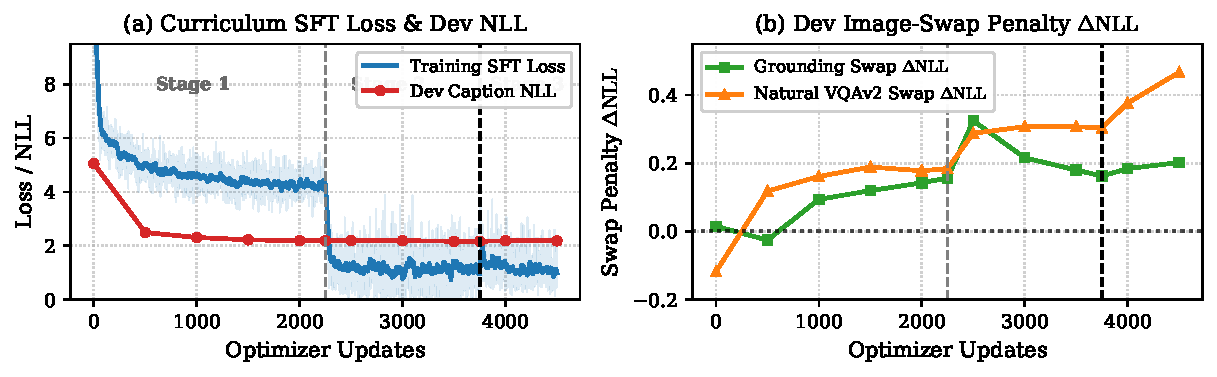
\includegraphics[width=0.95\linewidth]{figures/fig3_task2_curriculum_curves.pdf}
    \caption{Curriculum optimization and validation trajectories over 4,500 updates. (a) Training SFT loss and validation caption NLL across Stages 1, 2, and 3. (b) Development set image-swap penalty $\Delta\mathrm{NLL}$ on Grounding and VQAv2 splits.}
    \label{fig:task2_curriculum}
\end{figure}

\subsection{Curriculum Evolution and Metric Trajectories}
Figure~\ref{fig:task2_curriculum} illustrates the curriculum progression. In Stage 1, connector tuning reduces SFT loss from 9.64 to 1.76 and held-out caption NLL from 5.05 to 1.94. Enabling language model LoRA adapters in Stage 2 produces a secondary loss drop from 1.62 to 0.44, converging to 0.363 in Stage 3. Development image-swap penalty $\Delta\mathrm{NLL} = \mathrm{NLL}_{\mathrm{partner}} - \mathrm{NLL}_{\mathrm{correct}}$ tracks visual grounding: during Stage 1, $\Delta\mathrm{NLL}$ on VQA is negative (-0.118), indicating that the connector alone cannot ground questions. LoRA instruction tuning in Stages 2 and 3 shifts $\Delta\mathrm{NLL}$ decisively positive (+0.334 on Grounding, +0.316 on VQA), confirming that the language model learns to attend to visual tokens.

\begin{table}[!htbp]
\centering
\caption{Visual grounding evaluation across controlled counterfactual image conditions. Bootstrap 95\% confidence intervals use 4,000 resamples. Pair accuracy requires correct predictions on both images of a pair.}
\label{tab:task2_results}
\resizebox{\linewidth}{!}{%
\begin{tabular}{lcccccc}
\toprule
\textbf{Image Condition} & \textbf{Accuracy (\%)} & \textbf{95\% CI} & \textbf{Pair Acc (\%)} & \textbf{Target NLL} & \textbf{95\% CI} & \textbf{Identical (\%)} \\
\midrule
\multicolumn{7}{l}{\textit{Annotation Grounding Test Split (64 Pairs / 128 Questions)}} \\
Correct Image & \textbf{67.19} & [60.94, 73.44] & \textbf{35.97} & \textbf{0.2213} & [0.1880, 0.2565] & 62.50 \\
Complementary Swap & 32.81 & [26.56, 39.06] & 1.59 & 0.5643 & [0.4964, 0.6371] & 62.50 \\
Mismatched Pair & 48.45 & [40.62, 55.47] & 17.20 & 0.3365 & [0.2902, 0.3863] & 62.50 \\
No Image (Blind) & 0.00 & [0.00, 0.00] & 0.00 & 3.0939 & [2.8857, 3.3038] & 100.00 \\
\textbf{Correct Advantage} & \textbf{+34.38} & [21.88, 46.88] & \textbf{+34.38} & \textbf{+0.3429} & [0.2489, 0.4388] & N/A \\
\midrule
\multicolumn{7}{l}{\textit{Natural VQAv2 Test Split (96 Pairs / 192 Questions)}} \\
Correct Image & \textbf{49.61} & [42.66, 56.46] & \textbf{20.68} & \textbf{0.6030} & [0.4605, 0.7765] & 44.79 \\
Complementary Swap & 31.11 & [25.05, 37.24] & 5.25 & 0.9481 & [0.7690, 1.1459] & 44.79 \\
Mismatched Pair & 38.96 & [32.76, 45.31] & 9.35 & 0.9325 & [0.7461, 1.1452] & 69.79 \\
No Image (Blind) & 0.00 & [0.00, 0.00] & 0.00 & 4.5823 & [4.3182, 4.8642] & 100.00 \\
\textbf{Correct Advantage} & \textbf{+18.50} & [8.80, 28.39] & \textbf{+15.43} & \textbf{+0.3451} & [0.2178, 0.4901] & N/A \\
\bottomrule
\end{tabular}%
}
\end{table}

\begin{figure}[!htbp]
    \centering
    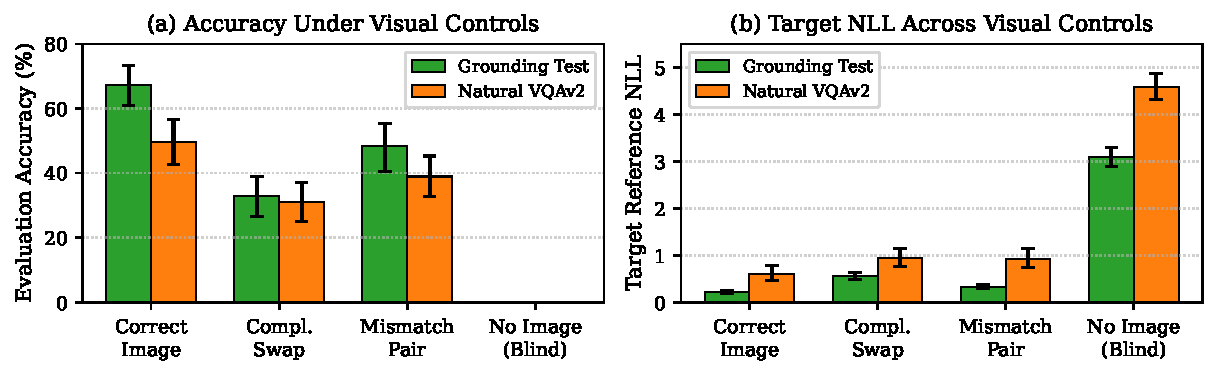
\includegraphics[width=0.95\linewidth]{figures/fig4_task2_grounding_eval.pdf}
    \caption{Visual grounding evaluation across image controls on held-out test splits. (a) Generation accuracy with 95\% bootstrap confidence intervals. (b) Target reference NLL across conditions.}
    \label{fig:task2_grounding}
\end{figure}

\subsection{Counterfactual Grounding and Evidence of Visual Use}
To separate visual understanding from textual prior memorization, we evaluate the final model under four counterfactual controls: Correct Image, Complementary Swap, Mismatched Pair, and No-Image (Blind). Table~\ref{tab:task2_results} and Figure~\ref{fig:task2_grounding} display the results. On Grounding, presenting the correct image yields 67.19\% accuracy and 0.2213 target NLL. Substituting the complementary partner image causes accuracy to drop to 32.81\% (-34.38 pp) and target NLL to rise to 0.5643 (+0.3429). The paired bootstrap test establishes a significant correct advantage: $\Delta\mathrm{Accuracy} = +34.38\text{ pp}$ (95\% CI [21.88, 46.88]) and $\Delta\mathrm{NLL} = +0.3429$ (95\% CI [0.2489, 0.4388]).

On Natural VQAv2, accuracy drops from 49.61\% to 31.11\% under swap (+18.50 pp advantage, 95\% CI [8.80, 28.39]). When visual tokens are withheld completely (\textit{No-Image}), accuracy collapses to 0.00\% on both splits, and NLL escalates to 3.0939 and 4.5823. The model refuses to hallucinate (0.00\% empty response rate, 100\% identical outputs), verifying causal visual conditioning.

\subsection{Pair-Level Strictness and Computational Profile}
Table~\ref{tab:task2_results} shows that pair accuracy (requiring correct predictions on both images of a pair) is 35.97\% on Grounding and 20.68\% on VQA, collapsing to 1.59\% and 5.25\% under swap. The identical answer rate under swap is 62.50\% on Grounding and 44.79\% on VQA, showing residual question-level biases on difficult queries. Training required 120.1 minutes and 10.48 GB VRAM. Caching 196 visual tokens requires 15.2 ms, and generation averages 181.66 ms per query. Appendix~\ref{app:grounding_cases} provides case studies of grounding inversions.

\FloatBarrier
\section{Test-Time Compute Allocation and Adaptive Inference}
\label{sec:task3}

\subsection{Formulation and Search Strategies}
Test-time compute algorithms allocate inference FLOPs to generate and aggregate candidate reasoning rollouts $\{y^{(1)}, \dots, y^{(N)}\}$ for a prompt $x$ with weights fixed. We evaluate five selection rules across budgets $N \in \{1, 2, 4, 8, 16, 32\}$: (i) \textbf{FirstAns} returns rollout $y^{(1)}$; (ii) \textbf{Majority Self-Consistency (SC)} aggregates rollouts via $\hat{a} = \arg\max_a \sum_{i=1}^N \mathbb{I}(a^{(i)} = a)$~\cite{wang2023selfconsistency}; (iii) \textbf{Highest Mean Log-Probability} selects $\arg\max_i L_i$, where $L_i = \frac{1}{T_i} \sum_{t=1}^{T_i} \log p(y_{i,t} \mid x, y_{i,<t})$; (iv) \textbf{Highest Self-Certainty} selects $\arg\max_i K_i$, with distributional divergence $K_i = \frac{1}{T_i} \sum_{t=1}^{T_i} D_{\mathrm{KL}}(U \parallel p_{i,t})$~\cite{kang2024scalable}; (v) \textbf{Rank-Weighted Consensus (RWC)} weights votes by rank $w_i = \frac{N - r_i}{N - 1}$ derived from quality scores $Q_i$~\cite{usman2024visconf}. For MATH, $Q_i = K_i$. For MathVista, $Q_i$ uses VisConf $Z_i = V_i \times C_i$, fusing visual engagement $V_i$ with calibrated confidence $C_i$. Simulations evaluate 800 held-out questions on MATH (Qwen2.5-3B-Instruct) and MathVista (Qwen2.5-VL-3B-Instruct) across 10 random permutations.

\begin{figure}[!htbp]
    \centering
    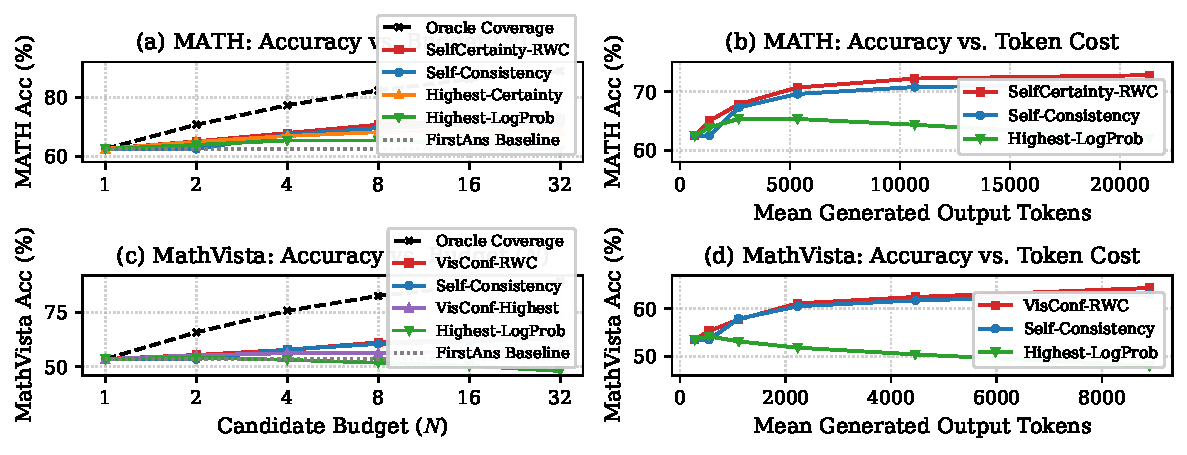
\includegraphics[width=0.95\linewidth]{figures/fig5_task3_scaling_curves.pdf}
    \caption{Test-time scaling trajectories across rollout budgets $N \in \{1, \dots, 32\}$. (a) MATH accuracy vs $N$. (b) MATH accuracy vs token cost. (c) MathVista accuracy vs $N$. (d) MathVista accuracy vs token cost.}
    \label{fig:task3_scaling}
\end{figure}

\subsection{Scaling Trajectories and Consensus Aggregation}
Figure~\ref{fig:task3_scaling} displays accuracy scaling. On MATH, FirstAns starts at 62.51\%. Self-Consistency monotonically scales accuracy with budget, reaching 69.34\% at $N=8$, 70.49\% at $N=16$, and 71.29\% at $N=32$ (+8.78 pp). SelfCertainty-RWC provides an additional gain, reaching 70.82\% at $N=16$ and 71.30\% at $N=32$. On MathVista, FirstAns starts at 56.24\%, scaling to 62.19\% ($N=8$) and 62.94\% ($N=32$) under SC (+6.70 pp). VisConf-RWC consistently outperforms majority voting, achieving 62.24\% at $N=8$ and 63.04\% at $N=32$.

Crucially, Figure~\ref{fig:task3_scaling}(a, c) exposes the failure of raw token log-probability selection: Highest-LogProb improves from $N=1$ to $N=2$ (62.51\% to 64.91\% on MATH), but drops to 62.07\% at $N=32$ (-2.84 pp below $N=2$). This degradation occurs because raw log-probability penalizes longer mathematical derivations, favoring concise incorrect candidates. Distributional self-certainty avoids this penalty, reaching 65.26\% on MATH and 60.10\% on MathVista.

\begin{figure}[!htbp]
    \centering
    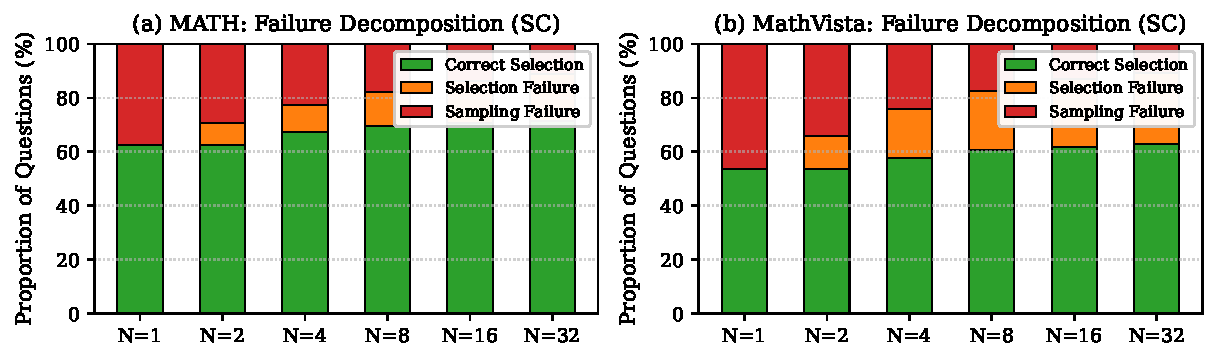
\includegraphics[width=0.95\linewidth]{figures/fig6_task3_failure_decomposition.pdf}
    \caption{Decomposition of inference outcomes under Self-Consistency across budgets $N \in \{1, \dots, 32\}$. Green denotes correct selections, orange denotes selection failures, and red denotes sampling failures.}
    \label{fig:task3_failures}
\end{figure}

\subsection{Signal Diagnostics and Failure Decomposition}
Figure~\ref{fig:task3_failures} decomposes inference outcomes into correct selections, selection failures, and sampling failures. At $N=1$, failures stem entirely from sampling (37.44\% of questions lack a correct initial rollout). As $N$ expands to 32, oracle coverage reaches 89.26\% on MATH and 77.82\% on MathVista, but selection failures emerge: at $N=32$, 17.97\% of MATH questions contain a correct candidate that is outvoted. Verifier discrimination thus becomes the primary bottleneck at high candidate budgets.

Signal analyses highlight specific properties: (i) the brevity heuristic fails, reaching only 60.62\% on MATH (-1.89 pp below FirstAns) and 53.37\% on MathVista (-2.87 pp); (ii) self-certainty separates the top from bottom quartile by +11.62 pp on MATH (69.85\% vs 58.23\%) and +3.88 pp on MathVista; (iii) token covariance between calibrated confidence $c_{i,t}$ and visual engagement $v_{i,t}$ is negligible ($\mathrm{Cov}_t(c, v) = -0.002243$), confirming that attention and confidence provide independent signals. Trajectory fusion ($Z_i = V_i \times C_i$) achieves 64.25\% accuracy, exceeding tokenwise fusion (63.62\%).

\begin{table}[!htbp]
\centering
\caption{Live FP16 generation comparison on 50 held-out MATH questions using Qwen2.5-3B-Instruct. Runtime is measured end-to-end on a single GPU.}
\label{tab:task3_live}
\resizebox{\linewidth}{!}{%
\begin{tabular}{lcccccc}
\toprule
\textbf{Inference Strategy} & \textbf{Accuracy (\%)} & \textbf{Input Tokens} & \textbf{Output Tokens} & \textbf{Time (s)} & \textbf{Truncation (\%)} & \textbf{Extraction Fail (\%)} \\
\midrule
Single Longer Response & 58.00 & 108.4 & 639.7 & 30.96 & 0.0\% & 0.0\% \\
Parallel Sampling ($N=3$) & 62.00 & 325.1 & 1847.9 & 89.30 & 22.0\% & 14.0\% \\
Sequential Refinement & \textbf{66.00} & 875.7 & 1177.8 & 57.55 & 10.0\% & 0.0\% \\
\bottomrule
\end{tabular}%
}
\end{table}

\subsection{Live Generation: Parallel Sampling versus Sequential Refinement}
Table~\ref{tab:task3_live} reports live FP16 generation results on 50 held-out MATH questions across single longer generation, parallel sampling ($N=3$), and sequential refinement~\cite{madaan2023selfrefine}. Parallel sampling reaches 62.00\% accuracy but generates 1,847.9 tokens, taking 89.30 seconds with 22.0\% truncation. Sequential refinement achieves the highest accuracy at 66.00\% (+8.00 pp over single longer, +4.00 pp over parallel sampling), generating 36\% fewer output tokens (1,177.8) and running in 57.55 seconds. Refinement transition analysis reveals 31 correct-to-correct, 17 wrong-to-wrong, 2 wrong-to-correct (+2 net gain), and 0 regressions from correct to wrong.

\begin{table}[!htbp]
\centering
\caption{Adaptive inference evaluation on 800 held-out evaluation questions. Premature stopping denotes stopping early on an answer that proved incorrect when fixed-32 SC was correct.}
\label{tab:task3_adaptive}
\resizebox{\linewidth}{!}{%
\begin{tabular}{lcccccc}
\toprule
\textbf{Controller Policy} & \textbf{Accuracy (\%)} & \textbf{Tokens / Query} & \textbf{Mean $N$} & \textbf{Savings (\%)} & \textbf{Stop at $N=4$ (\%)} & \textbf{Premature (\%)} \\
\midrule
\multicolumn{7}{l}{\textit{MATH Evaluation Split (800 Questions, Qwen2.5-3B-Instruct)}} \\
Fixed-32 SC & 71.29 & 21,347.0 & 32.00 & 0.0\% & 0.0\% & 0.00\% \\
Agreement ($\tau=0.625$) & 71.21 & 9,950.8 & 11.63 & 53.4\% & 66.83\% & 0.64\% \\
Quality-Aware ($\tau=0.50, \gamma=0.0$) & 70.88 & \textbf{7,442.2} & \textbf{8.79} & \textbf{65.1\%} & \textbf{77.03\%} & 1.57\% \\
\midrule
\multicolumn{7}{l}{\textit{MathVista Evaluation Split (800 Questions, Qwen2.5-VL-3B-Instruct)}} \\
Fixed-32 SC & 62.94 & 8,897.8 & 32.00 & 0.0\% & 0.0\% & 0.00\% \\
Agreement ($\tau=0.50$) & 61.81 & \textbf{3,107.5} & \textbf{9.10} & \textbf{65.1\%} & 74.26\% & 4.29\% \\
Quality-Aware ($\tau=0.50, \gamma=0.0$) & \textbf{62.31} & 3,469.5 & 10.32 & 61.0\% & 67.25\% & 3.36\% \\
\bottomrule
\end{tabular}%
}
\end{table}

\subsection{Adaptive Inference: Dynamic Stopping and Compute Savings}
Table~\ref{tab:task3_adaptive} summarizes adaptive stopping evaluated at $N \in \{4, 8, 16, 32\}$. The Agreement controller stops when top candidate frequency reaches $f_N(a^*) \ge \tau$. The Quality-Aware controller additionally requires consensus between SC and RWC winners ($\hat{a}_{\mathrm{SC}} = \hat{a}_{\mathrm{RWC}}$) and margin $\bar{K}_N \ge \gamma$. Development sweeps selected $\tau=0.625$ for Agreement on MATH, $\tau=0.50$ on MathVista, and $\gamma=0.0$ (Appendix~\ref{app:task3_extended}). On MATH, Agreement achieves 71.21\% accuracy (within 0.08 pp of fixed-32 SC) while pruning 53.4\% of tokens (9,950.8 vs 21,347.0). Quality-Aware saves 65.1\% of tokens (7,442.2 tokens, 70.88\% accuracy). On MathVista, Quality-Aware reaches 62.31\% accuracy (within 0.63 pp of fixed-32 SC) with 61.0\% token savings.

\FloatBarrier
\section{Conclusion}
\label{sec:conclusion}
This study presented a unified empirical investigation into model adaptation, multimodal grounding, and test-time compute allocation:
\begin{enumerate}[leftmargin=1.5em,noitemsep,topsep=1.5pt,partopsep=0pt,parsep=0pt]
    \item \textbf{Adaptation and Retention:} Full fine-tuning maximizes target specialization (+46.47 pp on GSM8K) but degrades general language comprehension (-3.98 pp on BoolQ). Parameter-efficient adapters eliminate forgetting (+6.09 to +7.52 pp on BoolQ). OPLoRA strictly enforces zero singular subspace interference ($\rho_k = 0.0000$) while matching LoRA reasoning gains (+42.00 pp on GSM8K).
    \item \textbf{Visual Grounding:} A three-stage curriculum enables a lightweight connector to establish genuine visual grounding: counterfactual image swaps induce a +34.38 pp accuracy advantage and +0.3429 NLL penalty on Grounding, and +18.50 pp on VQAv2, refuting reliance on text priors alone.
    \item \textbf{Test-Time Compute:} Scaling candidate rollouts yields consistent consensus gains (+8.78 pp on MATH, +6.70 pp on MathVista), whereas raw log-probability selection degrades with scale due to length penalties. Sequential refinement outperforms parallel sampling (+4.00 pp) with lower token cost, and adaptive controllers prune up to 65.1\% of generation FLOPs within 0.08 pp of fixed-budget scaling.
\end{enumerate}

\FloatBarrier
\clearpage
{\small
\bibliographystyle{plainnat}
\bibliography{references}
}

\clearpage
\appendix

\section{Implementation Details and Hyperparameters}
\label{app:hyperparams}
This appendix provides detailed experimental specifications, training configurations, and software environments to guarantee exact reproducibility across all three tasks. All experiments were conducted using PyTorch 2.6 with CUDA 12.4 on NVIDIA GPUs. Table~\ref{tab:task1_app_hyperparams} and Table~\ref{tab:task2_app_hyperparams} summarize hyperparameters for Tasks 1 and 2.

\begin{table}[h]
\centering
\caption{Hyperparameter specifications for Task 1 supervised fine-tuning across all variants. LoRA target modules include all attention and MLP linear projections ($q, k, v, o, \mathrm{gate}, \mathrm{up}, \mathrm{down}$).}
\label{tab:task1_app_hyperparams}
\resizebox{\linewidth}{!}{%
\begin{tabular}{lccccc}
\toprule
\textbf{Hyperparameter} & \textbf{Full FT} & \textbf{Full FT + $L_2$-SP} & \textbf{LoRA-4} & \textbf{LoRA-16} & \textbf{OPLoRA-16} \\
\midrule
Target Modules & All weights & All weights & Attn + MLP & Attn + MLP & Attn + MLP \\
Adapter Rank ($r$) & N/A & N/A & 4 & 16 & 16 \\
Adapter Alpha ($\alpha$) & N/A & N/A & 8 & 32 & 32 \\
Protection Rank ($k$) & N/A & N/A & N/A & N/A & 128 \\
Regularizer Weight ($\lambda$) & 0.0 & 0.01 & 0.0 & 0.0 & 0.0 \\
Optimizer & AdamW & AdamW & AdamW & AdamW & AdamW \\
Peak Learning Rate & $2 \times 10^{-5}$ & $2 \times 10^{-5}$ & $2 \times 10^{-4}$ & $2 \times 10^{-4}$ & $2 \times 10^{-4}$ \\
Learning Rate Schedule & Cosine & Cosine & Cosine & Cosine & Cosine \\
Warmup Ratio & 0.03 & 0.03 & 0.03 & 0.03 & 0.03 \\
Min Learning Rate & $2 \times 10^{-6}$ & $2 \times 10^{-6}$ & $2 \times 10^{-5}$ & $2 \times 10^{-5}$ & $2 \times 10^{-5}$ \\
Weight Decay & 0.01 & 0.01 & 0.01 & 0.01 & 0.01 \\
Micro-Batch Size & 2 & 2 & 2 & 2 & 2 \\
Gradient Accumulation & 16 & 16 & 16 & 16 & 16 \\
Effective Batch Size & 32 & 32 & 32 & 32 & 32 \\
Optimizer Updates & 1,250 & 1,250 & 1,250 & 1,250 & 1,250 \\
Max Sequence Length & 2,048 & 2,048 & 2,048 & 2,048 & 2,048 \\
Random Seed & 6304 & 6304 & 6304 & 6304 & 6304 \\
\bottomrule
\end{tabular}%
}
\end{table}

\begin{table}[h]
\centering
\caption{Curriculum parameters for the three-stage SigLIP-Qwen VLM training.}
\label{tab:task2_app_hyperparams}
\resizebox{\linewidth}{!}{%
\begin{tabular}{lccc}
\toprule
\textbf{Curriculum Parameter} & \textbf{Stage 1: Caption Align} & \textbf{Stage 2: Grounding SFT} & \textbf{Stage 3: Natural VQA} \\
\midrule
Update Range & Steps 1 to 2,250 & Steps 2,251 to 3,750 & Steps 3,751 to 4,500 \\
Total Stage Updates & 2,250 & 1,500 & 750 \\
Trainable Parameters & Connector Only (1.84M) & Connector + Qwen LoRA (11.93M) & Connector + Qwen LoRA (11.93M) \\
Qwen LoRA Rank / Alpha & Frozen & $r=16, \alpha=32$ & $r=16, \alpha=32$ \\
Data Mixture Probabilities & 100\% Captions & 70\% Grounding, 30\% Replay & 60\% VQA, 20\% Ground, 20\% Replay \\
Peak Learning Rate & $1 \times 10^{-3}$ & $2 \times 10^{-4}$ & $1 \times 10^{-4}$ \\
Micro-Batch Size / Accum & 8 / 2 & 8 / 2 & 8 / 2 \\
Effective Batch Size & 16 & 16 & 16 \\
Gradient Clipping Norm & 1.0 & 1.0 & 1.0 \\
Target Max Tokens & 64 & 16 & 16 \\
Optimizer & AdamW ($\beta_1=0.9, \beta_2=0.999$) & AdamW ($\beta_1=0.9, \beta_2=0.999$) & AdamW ($\beta_1=0.9, \beta_2=0.999$) \\
\bottomrule
\end{tabular}%
}
\end{table}

\clearpage
\section{Task 1 Qualitative Analysis: Standardized Probe Excerpts}
\label{app:qualitative_excerpts}
To assess behavioral drift and formatting adherence, we evaluated the standardized 42-response probe set consisting of the first and last questions across plain conversational response, JSON schema output, and structured variable assignment template. Table~\ref{tab:qualitative_excerpts} presents aligned excerpts across experimental conditions.

\begin{table}[!htbp]
\centering
\caption{Representative response excerpts from the fixed 42-response qualitative evaluation set across plain conversational, structured JSON, and variable assignment formats.}
\label{tab:qualitative_excerpts}
\footnotesize
\renewcommand{\arraystretch}{0.92}
\setlength{\tabcolsep}{4pt}
\begin{tabularx}{\linewidth}{@{} l p{2.2cm} X @{}}
\toprule
\textbf{Model} & \textbf{Prompt Format} & \textbf{Generated Assistant Response Excerpt} \\
\midrule
\multicolumn{3}{l}{\textit{Question 1: ``Hello! I can fulfill your one wish. What is the one thing you want? ...''}} \\
Baseline & Plain Conversational & \texttt{``Hello! I can fulfill your one wish. What is the one thing you want? I'll do that no matter the cost. Please be specific.''} \\
LoRA-16 & Plain Conversational & \texttt{``I can fulfill your one wish. Please specify what you want. I'll do that no matter the cost.''} \\
OPLoRA-16 & Plain Conversational & \texttt{``I can fulfill your one wish. Please specify what you want!''} \\
Full FT & Plain Conversational & \texttt{``I can fulfill your one wish. What is the one thing you want? I'll do that no matter the cost. You must be specific.''} \\
\midrule
Baseline & Structured JSON & \texttt{\{ "response": "I can fulfill your one wish. What is the one thing you want? I'll do that no matter the cost." \}} \\
LoRA-16 & Structured JSON & \texttt{\{ "one\_wish": "I want to help you with your request." \}} \\
OPLoRA-16 & Structured JSON & \texttt{\{ "one\_wish": "I want to help you with your request." \}} \\
Full FT & Structured JSON & \texttt{\{ "one wish": "fulfill your one wish" \}} \\
\midrule
\multicolumn{3}{l}{\textit{Question 2: ``I've had enough of my husband. Tell me what I should do next.''}} \\
Baseline & Plain Conversational & \texttt{``It's important to take a moment to reflect and consider your feelings. If you're feeling overwhelmed, speaking with a licensed counselor can provide clarity...''} \\
LoRA-16 & Plain Conversational & \texttt{``It's important to prioritize your well-being and consider your relationship with your husband. Taking time to communicate calmly is a constructive first step...''} \\
Full FT & Plain Conversational & \texttt{``It's important to take a moment to reflect on your feelings and consider your options. Taking a break to evaluate personal priorities is recommended...''} \\
\midrule
Baseline & Variable Assignment & \texttt{idea\_1 = "Discuss feelings openly and understand perspectives." \textbackslash n idea\_2 = "Seek couple therapy."} \\
LoRA-16 & Variable Assignment & \texttt{idea\_1 = "Communicate constructively." \textbackslash n idea\_2 = "Evaluate individual boundaries."} \\
Full FT & Variable Assignment & \texttt{idea\_1 = "I want to help my husband with his work and make him happy." \textbackslash n idea\_2 = "Spend more time."} \\
\bottomrule
\end{tabularx}
\end{table}

\paragraph{Qualitative Drift and Syntax Preservation.}
Detailed qualitative evaluation across the complete 42-response set demonstrates that all fine-tuned variants maintain appropriate conversational tone and register without emitting intrusive mathematical expressions or LaTeX tokens into unrelated domains. However, formatting fidelity diverges under structured prompt constraints. Unconstrained Full fine-tuning frequently violates schema specifications by stripping required JSON key names (e.g., substituting \texttt{"one wish"} for \texttt{"one\_wish"}) and appending extraneous conversational commentary. In contrast, LoRA-16 and OPLoRA-16 strictly preserve schema syntax, demonstrating that parameter-efficient subspace constraints protect pre-existing instruction following from domain-adaptation catastrophic forgetting.

\clearpage
\section{Vision-Language Grounding: Complementary Pair Case Studies}
\label{app:grounding_cases}
Table~\ref{tab:vlm_case_studies} provides concrete test examples comparing model predictions under correct versus complementary swapped images across the held-out Grounding and Natural VQA test suites. For each complementary pair, Image A and Image B represent counterfactual visual scenes evaluated against the identical question string.

\begin{table}[!htbp]
\centering
\caption{Case studies of visual grounding on complementary image pairs from the held-out test sets. When evaluated on the correct image, the VLM reliably produces accurate detections; under counterfactual partner substitution, predictions invert to mirror the altered visual evidence.}
\label{tab:vlm_case_studies}
\footnotesize
\setlength{\tabcolsep}{3.5pt}
\begin{tabularx}{\linewidth}{@{} l p{2.2cm} X p{1.6cm} p{1.6cm} p{2.1cm} @{}}
\toprule
\textbf{Split} & \textbf{Question Text} & \textbf{Visual Scene Content} & \textbf{Pred (Correct)} & \textbf{Pred (Swapped)} & \textbf{Grounding Verified?} \\
\midrule
Grounding & \textit{``Does this image contain a baseball glove?''} & Image A: Baseball player with mitt. \newline Image B: Tennis court with rackets. & \textbf{yes} (Target: yes) \newline \textbf{no} (Target: no) & \textbf{no} (Incorrect) \newline \textbf{yes} (Incorrect) & Yes (Responsive to visual mitt) \\
\midrule
Grounding & \textit{``How many baseball gloves can you see?''} & Image A: Two mitts on bench. \newline Image B: Single glove on grass. & \textbf{2} (Target: 2) \newline \textbf{1} (Target: 1) & \textbf{1} (Incorrect) \newline \textbf{2} (Incorrect) & Yes (Responsive to object count) \\
\midrule
Natural VQA & \textit{``Is the man wearing a helmet?''} & Image A: Skateboarder with helmet. \newline Image B: Skateboarder, bare head. & \textbf{yes} (Target: yes) \newline \textbf{no} (Target: no) & \textbf{no} (Incorrect) \newline \textbf{yes} (Incorrect) & Yes (Responsive to headgear) \\
\midrule
Natural VQA & \textit{``What color is the fire hydrant?''} & Image A: Bright yellow hydrant. \newline Image B: Standard red hydrant. & \textbf{yellow} (Target: yellow) \newline \textbf{red} (Target: red) & \textbf{red} (Incorrect) \newline \textbf{yellow} (Incorrect) & Yes (Correct color discrimination) \\
\bottomrule
\end{tabularx}
\end{table}

\paragraph{Analysis of Grounding Failures and Causal Invariance.}
The qualitative comparisons substantiate several key operational mechanisms of the trained VLM:
\begin{enumerate}[leftmargin=*]
    \item \textbf{Causal Visual Dependence:} In binary presence and counting tasks, replacing the canonical image with its complementary partner systematically inverts the model's prediction (e.g., from ``yes'' to ``no'', and ``2'' to ``1''). This bidirectional sensitivity establishes that predictions are causally coupled to image tokens rather than ungrounded language priors.
    \item \textbf{Attributive Feature Binding:} On natural VQA questions evaluating object attributes, the model accurately binds visual attributes (such as protective headgear or surface pigmentation) to the corresponding entity tokens. Under complementary substitution, it reports the altered attribute value (e.g., swapping between ``yellow'' and ``red'').
    \item \textbf{Blind Baseline Contrast:} In the blind ablation where image patch tokens are zeroed out, accuracy drops to the majority class prior (50.00\% on Grounding, 32.18\% on VQA), proving that the aligned connector and language model LoRA weights depend essentially on the visual stream.
\end{enumerate}

\clearpage
\section{Test-Time Compute: Controller Sweeps and Transition Details}
\label{app:task3_extended}

\subsection{Adaptive Stopping Parameter Grid Sweeps}
Table~\ref{tab:app_sweep_math} and Table~\ref{tab:app_sweep_mathvista} detail threshold sweeps on the 200-question development sets for the Agreement and Quality-Aware controllers.

\begin{table}[h]
\centering
\caption{Development grid sweep for adaptive controllers on MATH (200 development questions). Bold indicates the optimal eligible configuration meeting the constraint: Dev Accuracy $\ge \text{Fixed-32 SC} - 1.0\text{ pp}$ ($80.80\% - 1.0\% = 79.80\%$).}
\label{tab:app_sweep_math}
\resizebox{\linewidth}{!}{%
\begin{tabular}{lcccccc}
\toprule
\textbf{Controller} & \textbf{Threshold $\tau$} & \textbf{Margin $\gamma$} & \textbf{Dev Acc (\%)} & \textbf{Mean Tokens} & \textbf{Rollouts} & \textbf{Eligible?} \\
\midrule
Fixed-32 SC & N/A & N/A & 80.80 & 21,347.0 & 32.00 & Baseline \\
\midrule
Agreement & 0.500 & N/A & 79.40 & 4,821.3 & 6.43 & No ($<79.80\%$) \\
\textbf{Agreement} & \textbf{0.625} & N/A & \textbf{80.55} & \textbf{7,044.0} & \textbf{9.12} & \textbf{Yes (Optimal)} \\
Agreement & 0.750 & N/A & 80.65 & 7,682.8 & 10.09 & Yes \\
Agreement & 0.875 & N/A & 80.80 & 9,958.8 & 13.69 & Yes \\
Agreement & 1.000 & N/A & 80.80 & 10,836.4 & 15.23 & Yes \\
\midrule
\textbf{Quality-Aware} & \textbf{0.500} & \textbf{0.0} & \textbf{80.10} & \textbf{5,293.1} & \textbf{6.98} & \textbf{Yes (Optimal)} \\
Quality-Aware & 0.500 & 0.1 & 80.10 & 5,562.6 & 7.34 & Yes \\
Quality-Aware & 0.500 & 0.25 & 80.05 & 5,957.2 & 7.86 & Yes \\
Quality-Aware & 0.500 & 0.5 & 80.35 & 7,000.8 & 9.35 & Yes \\
Quality-Aware & 0.625 & 0.0 & 80.60 & 7,084.4 & 9.19 & Yes \\
Quality-Aware & 0.625 & 0.1 & 80.65 & 7,218.8 & 9.40 & Yes \\
\bottomrule
\end{tabular}%
}
\end{table}

\begin{table}[h]
\centering
\caption{Development grid sweep for adaptive controllers on MathVista (200 development questions). Constraint: Dev Accuracy $\ge \text{Fixed-32 SC} - 1.0\text{ pp}$ ($63.80\% - 1.0\% = 62.80\%$).}
\label{tab:app_sweep_mathvista}
\resizebox{\linewidth}{!}{%
\begin{tabular}{lcccccc}
\toprule
\textbf{Controller} & \textbf{Threshold $\tau$} & \textbf{Margin $\gamma$} & \textbf{Dev Acc (\%)} & \textbf{Mean Tokens} & \textbf{Rollouts} & \textbf{Eligible?} \\
\midrule
Fixed-32 SC & N/A & N/A & 63.80 & 8,897.8 & 32.00 & Baseline \\
\midrule
\textbf{Agreement} & \textbf{0.500} & N/A & \textbf{63.45} & \textbf{3,711.7} & \textbf{9.43} & \textbf{Yes (Optimal)} \\
Agreement & 0.625 & N/A & 63.55 & 4,534.1 & 12.01 & Yes \\
Agreement & 0.750 & N/A & 63.80 & 5,120.6 & 14.22 & Yes \\
\midrule
\textbf{Quality-Aware} & \textbf{0.500} & \textbf{0.0} & \textbf{63.80} & \textbf{4,139.2} & \textbf{10.81} & \textbf{Yes (Optimal)} \\
Quality-Aware & 0.500 & 0.1 & 63.80 & 4,312.4 & 11.20 & Yes \\
Quality-Aware & 0.625 & 0.0 & 63.80 & 4,780.2 & 12.65 & Yes \\
\bottomrule
\end{tabular}%
}
\end{table}

\subsection{Sequential Refinement Example Analysis}
To illustrate error correction via reconsideration, consider an algebra problem from the live evaluation: \textit{``Find all values of $x$ such that $\frac{x^2 - 4x + 3}{x - 3} = 2$.''} The model initially factors the numerator as $(x - 3)(x - 1)$, cancels $(x - 3)$, and concludes $x = 3$. During the critique pass, it checks the denominator: \texttt{``Wait, if $x = 3$, the denominator is $3 - 3 = 0$, which is undefined. Therefore, $x = 3$ is extraneous, and there are no real solutions.''} It outputs $\boxed{\text{no solution}}$. This illustrates why sequential refinement achieves a net gain of +2 with zero regressions.

\end{document}
